%%%% fs-run-mapreduce Optimistic collision management
\label {fs-collision}

\subsection{Existing solutions}

\subsection{Optimistic approach}

As it was defined previously, only the grouping operation maintains a state and the state depends on the order of incoming items. Because of asynchrony and the possible existence of multiple paths between two nodes it is hard to deliver the right order.

In order to address this issue, we accept the fact that grouping can produce incorrect tuples. However, we guarantee that all correct tuples are eventually produced. The correctness of tuple means that this tuple would be generated if the order assumption was satisfied. 

To eventually produce all correct tuples, we use an approach called {\it replay}. If an item arrives the grouping operation, according to the meta-information order, nothing is replayed and only the most recent window is produced. However, if an item is out-of-order, it is inserted in the bucket at the correct location, and all tuples, which contain this element, are reproduced. Thereby, replay guarantees that eventually all correct tuples are generated. At the same time, for tuples, that has been produced but became invalid, {\it tombstones} are sent.

Tombstones are ordinal data items but with a special flag in its meta-information. This flag means that tuples with such meta-information are invalid, and they should not leave the system. Tombstones have the same payloads as invalid items in order to go along the same path in the computational pipeline.

The example of replay is shown in Figure~\ref{grouping-replaying}, The green item is out-of-order. The output consists of the new valid items {\it (1, 2) and (2, 3)}, and the tombstone {\it (1, 3)} for the previously generated item.

\begin{figure}[htbp]
  \centering
  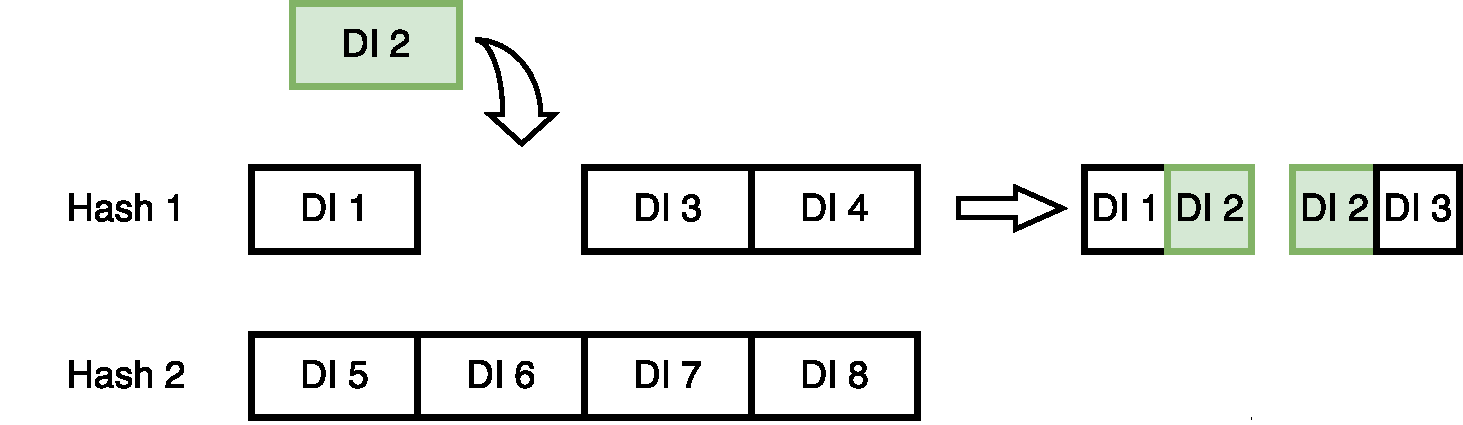
\includegraphics[width=0.48\textwidth]{pics/grouping-replaying}
  \caption{The replay in groupig with window = 2. The new items are generated on insertion}
  \label {grouping-replaying}
\end{figure}

In the case of the right order of input items, there are no redundant items produced.

The barrier filters out invalid elements, when corresponding tombstones arrive. It is partially flushed for some meta-information interval when there is a guarantee that there are no any out-of-order items and tombstones further up the stream for this range. The exact technique for providing such guarantee is defined in Section~\ref{fs-impl}.

\subsection{Advantages and limitations}

The proposed architecture's performance depends on how often reorderings are observed during the runtime. In the case when the order naturally preserved there is almost no overhead: when the watermark arrives, all computations are already done. The probability of reordering could be managed on a business-logic level and optimized by the developer. In experiments section it is shown that the computational nodes count is one of such parameters. Regarding the weaknesses, this method can generate additional items, which lead to extra network traffic and computations. Experiments, which are shown in the section~\ref{fs-experiments-section} demonstrate that the number of extra items is low.

